\chapter{Related Work}
  Nowadays, Many scholars from all around the world have submitted research 
  projects relating to the topic of turning sign language into text, 
  using a variety of methodologies and perspectives.
  % TODO: Change paper
  In which, two main approaches can be mentioned as follows:
  \begin{itemize}
    \item Glove based approaches:
    With this approach, it requires deaf and mute people to wearing a sensor glove. When user
    has any different action or gesture, these sensor will be recorded. After that, data from
    sensor will analyze by analyzer component and return the output for user.
    \item Vision based approaches:
    With this approach, image processing algorithms will be applied to be able to determine
    hand position, gestures and movements of the hand. The user will not have to wear necessary
    equipment like glove based approaches, which is convenient for user. However, with using
    library or algorithms of image processing, we need to deal with worst quality output, which is
    greatly affected by this algorithms.
  \end{itemize}

  Early work, with vision based approach, they used several types of
  image processing algorithm to build a feature vectors base on a single RGB image of hand.
  In this paper "Real-time sign language recognition using a consumer depth camera",
  with using multi-layered random forest (MLRF), not only it allows they recognize hand signs
  correctly, but also minimize training time and effort. Or in this paper "Sign Language Translation in Urdu/Hindi Through
  Microsoft Kinect", sign language can be recognize by an auxiliary equipment: Microsoft Kinect (see figure \ref{fig:Chap2-MS-Kinect}), which captures
  the signs of the deaf person, after that, through the computer system, they can detect what does deaf people say.

  \begin{figure}[H]
    \centering
    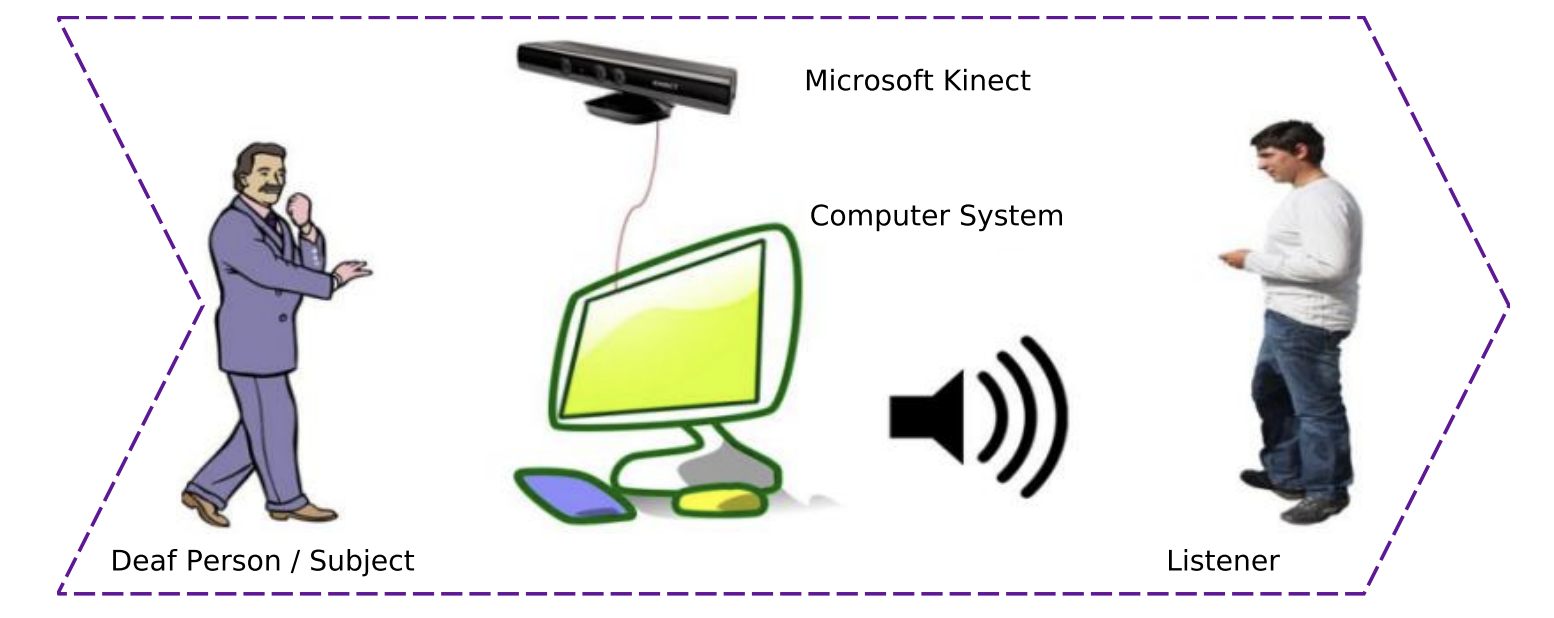
\includegraphics[width=\textwidth]{img/Chap2/MS-Kinect.png}
    \caption{Using Microsoft Kinect in translating sign language}
    \label{fig:Chap2-MS-Kinect}
  \end{figure}

  Beside vision based approach, glove based approach has many relevant research. This paper “The Language of Glove: Wireless gesture
  decoder with low-power and stretchable hybrid electronics” introduces the way to convert American
  Sign Language (ASL) alphabet into text and display it on a computer 
  or smartphone (see figure \ref{fig:Chap2-Glove-Base}). With sensor glove, they can detect which hand gesture is
  performed and sent the result to smartphone via bluetooth. The sign language
  interprets into some text and displays on the digital display screen.
  Both this approach is useful in the real world for the deaf and dumb 
  who are unable to converse with normal people.

  \begin{figure}[H]
    \centering
    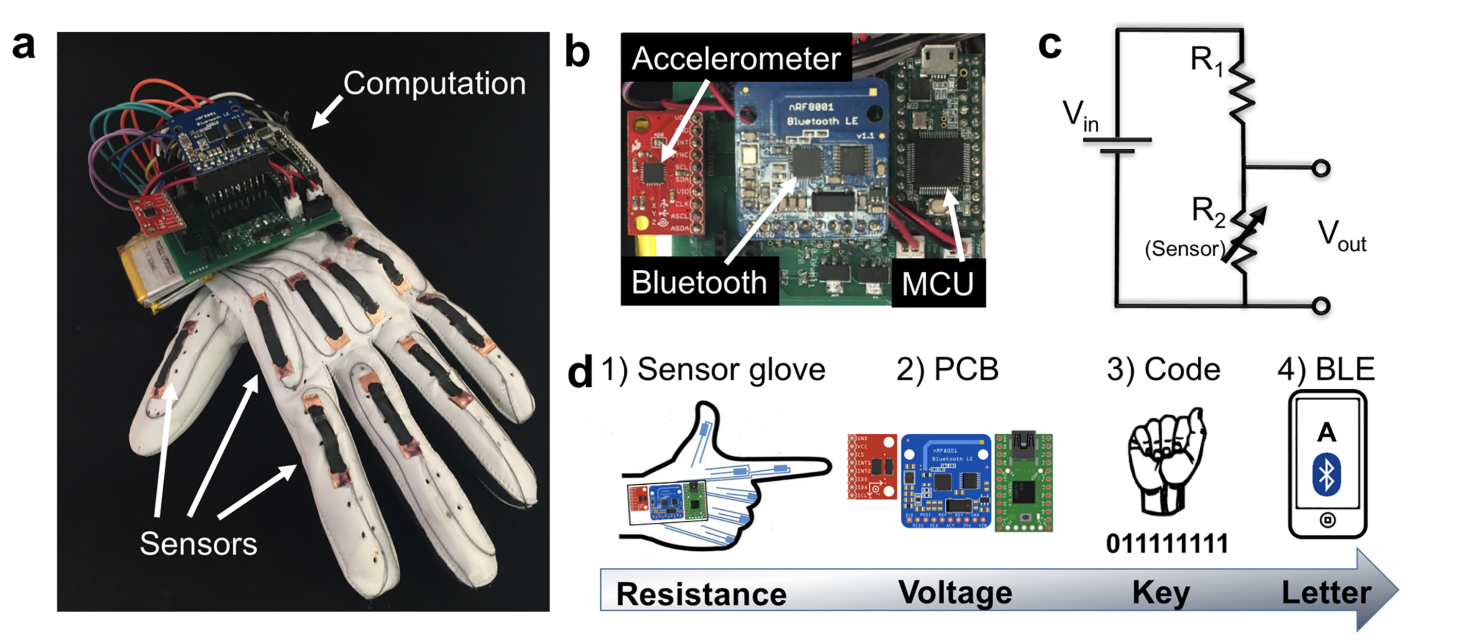
\includegraphics[width=\textwidth]{img/Chap2/Glove-Based.png}
    \caption{Glove based approach in translating sign language}
    \label{fig:Chap2-Glove-Base}
  \end{figure}

  % TODO: Fix grammar for this
  With both approaches above, it has some problems, that is, they can only recognize 
  a very small number of words, like an alphabet, number or some word with easily hand shape and no motion .
  However, in sign language, it not easy, there will be many words 
  that use the same hand shape but will differ in many characteristics, such as position 
  and direction. To our knowledge, there is currently no model that can handle the 
  conversion of sign language flexibly and conveniently for the deaf-mute, helping them 
  to communicate effectively and naturally. Therefore, by applying appropriate 
  technologies, the authors carry out this graduation thesis with the goal of breaking down 
  the barriers between deaf-mute people and normal people, helping them to become self-sufficient. 
  more confident in daily communication.

